\chapter{Introduction}
In Machine Learning course we will introduce principles and models that makes possible to make prediction
given data, even also if we don't know how to obtain result.\newline
In early ages of Computer Science to obtain some results we have to develop some algorithms to solve that 
but sometimes we don't have a knowledge of how to obtains some results but we have a lot of data and we 
uses in ML this data to infer a model which allows the generalization and be able to provide accurate response
on new data.\newline
In \cite{aiMagazine} Poggio and Shelton says that the problem of learning is arguably at the very core of 
the problem of intelligence, both biological and artificial.

ML can be useful as predictive models when we have no (or poor) theory, a lack in knowledge to how to explain
a phenomenon and we have uncertain, noisy or incomplete data, and also it is request when we use ML models 
to have a source of training experience and a tolerance on the precision of results.\newline
The ML studies and proposes methods to build (infer) dependencies/functions/hypotheses from examples
of observed data, that fits the know examples and able to generalize, with reasonable accuracy for new data,
under statistical and computational conditions and criteria.

Some examples of application of ML are real-world systems, like human computer interface and search engine,
pattern recognition (face and speech recognition), Computer Vision, Natural Language Processing and so on.

In figure \ref{img:mlProcess} it is possible to note all components of a ML process that we will analyzed now:
\begin{description}
    \item [Data: ] represent the available facts (experience) and can helps to capture the structure
                   of the analyzed objects.\newline
                   There different type of data, from numerical value to graph element, to complex data
                   from other fields like DNA elements.\newline
                   Data can suffer from $3$ problems that will be now briefly introduced:
                   \begin{enumerate}
                        \item \emph{Noise}: addition of external factors to the stream of target information (signal),
                              due to randomness in the measurements, not due to the underlying law.
                        \item \emph{Outliers}: unusual data values that are not consistent with most
                                               observations, due to abnormal measurements errors.\newline
                                               In preprocessing phase we should reduce or completely remove 
                                               outlier that can will create unrepresentive result in modelation.
                        \item \emph{Feature selection}: selection of a small number of informative features and it
                                    can provide an optimal input representation for a learning problem.
                   \end{enumerate}
    \item [Task: ] defines the purpose of the application and it is the knowledge that we want to achieve
                   (is it pattern in DM or model in ML) and we have two different type of task, both important:
                   \begin{description}
                        \item [Predictive: ] is the function approximation and it composed 
                                             by Classification and Regression.
                        \item [Descriptive: ] has objective to find subsets or groups of unclassified data 
                        and it is composed by cluster analysis and association rules.
                   \end{description}
                   Task can be also suddivised by the present or absent of precedent result:
                   \begin{itemize}
                        \item \emph{Supervised learning: } Given Training examples as $<input, output> = (x, y)$
                               for an unknown function $f$, known only at the given points of example) we have also
                               a target value, the desiderate value of y, given by the teacher according to $f(x)$
                               to label the data and we would like to find a good approximation of $f$ that can 
                               be used to predict $y'$ on unseen data $x'$.\newline
                               If we have that $y$ has discrete value output we have a \emph{Classification} task
                               instead if we have continuous output values we have a \emph{Regression} task.

                        \item \emph{Unsupervised Learning:} there is no label data from teacher and we only
                              have a set of unlabeled data $x$ and we want to find natural groupings inside
                              the set of data; \emph{Clustering} is an example of an Unsupervised learning task.

                        \item \emph{Semisupervised Learning: } combines both labeled and unlabeled examples
                              to generate an appropriate function or classifier.

                        \item \emph{Reinforcement Learning: } is the adaptation in autonomous systems and 
                              ML algorithms learns a policy of how to act given an observation of the
                              world and every action has some impact in the environment, so the
                              environment provides feedback that guides the learning algorithm.
                   \end{itemize}
    \item [Model: ] aims to capture/describes the relationships among the data (on the basis of the task)
                    by a “language”, related to the representation used to get knowledge.\newline
                    It defines the class of functions that the learning machine can implement (hypothesis space),
                    set of functions $h(x, w)$, where $w$ is the (abstract) parameter.\newline
                    \emph{Hypothesis function} is a proposed function $h$ that we believed to be similar to $f$ 
                    and it is an expression in a given language that describes the relationship among data.\newline
                    Unfortunately there is no universal “best” learning method, so if an algorithm achieves
                    superior results on some problems, it must pay with inferiority on other problems;
                    in this sense there is no free lunch.

    \item [Learning Algorithms: ] is an (Heuristic) search through the hypothesis space H of the best hypothesis
                                  and typically searching for the h with the minimum “error”, where 
                                  free parameters of the model are fitted to the task at hand.\newline
                                  $H$ may not coincide with the set of all possible functions and the
                                  search can not be exhaustive: we need to make assumptions and we will
                                  see the rule of \emph{Inductive bias}.
    
    \item [Loss function: ] is the union of Task and Model and it is a good approximation to $f$ from examples.\newline
                            We use a inner loss function $L(h(x), y)$ to measure the distance between $h(x)$ and $y$,
                            so if we have an high value it meanst that we have a poor approximation; this loss 
                            function changes for different tasks so we have always to define it.\newline
                            The Error (or Risk or Loss) is an expected value of this $L$ defined as 
                            \[ E(w) = \frac{1}{l} \sum _{p=1}^l L(h(x_p), y) \]
                            A possible classifications of common learning tasks specifying the 
                            (changing of the) nature of the loss function (in particular of L),
                            output and hypothesis space.
                            
                            \begin{defi}[overfitting]
                            We have that learner \emph{overfit} the data if it outputs a hypothesis $h \in H$
                            having true error $R$ and empirical error $E$, but there is another hypothesis $h' \in H$
                            having $E' > E$ and $R' < R$.
                            \end{defi}
                            In figure \ref{img:overfitting} we can see the effect of overfitting in polynomial
                            fitting, with also in figure \ref{img:coefficients} it possible to note the 
                            coefficients of our polynomial fitting.
    \item [Validation: ] evaluation of performances for ML systems gives a predictive accuracy and we have
                         that the performance on training data provide an overoptimistic evaluation.\newline
                         Validation has $2$ aims:
                         \begin{enumerate}
                            \item \emph{Model selection} where we estimating the performance (generalization error)
                                  of different learning models in order to choose the best one (to generalize) and 
                                  this includes search the best hyper-parameters of your model and returns a model.
                            \item \emph{Model assessment}, after we have chosen a final model,
                                  estimating/evaluating its prediction error/ risk (generalization error)
                                  on new test data (measure of the quality/performance of the ultimately chosen model)
                                  and it returns an estimation.
                         \end{enumerate}
                         A good rule is to keep a separation between goals and use separate datasets to validate
                         and test our model, so we should have $3$ dataset: a training set, to find the best 
                         hypothesis, a validation set for model selection and in the end a external unseen 
                         test dataset to estimate our prediction error.
                            
                         If we have infinite data there are not problem, but we have only a small amount of data
                         we have to choose how to create these $3$ datasets so we present now some technique
                         to do validation, that will be extended later during the course:
                         \begin{description}
                             \item [Hold-out Cross Validation: ] we partition dataset $D$ into $3$ disjoint sets
                                    training set $TR$, validation set $VL$ and test set $TS$, as we can see
                                    in figure \ref{img:hold-out} and in figure \ref{img:dataset} we can see
                                    the purpose of each dataset.
                             
                            \item [K-fold Cross Validation: ] Hold CV make an insufficient use of data so we 
                                  split the dataset $D$ into $k$ mutually exclusive subsets $D_1, D_2, \dots, D_k$
                                  to train the learning algorithm on $D - D_i$ and test it on $D_i$ and it uses
                                  all the data for training and validation/testing.
                        \end{description}

                        \begin{figure}
                            \caption{Representation of dataset in Hold-out validation}
                            \label{img:hold-out}
                            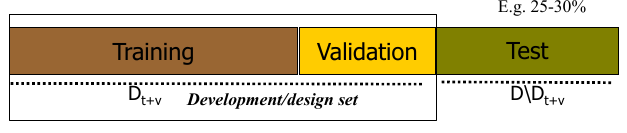
\includegraphics[width=\textwidth]{images/holdOut}
                        \end{figure}

                        \begin{figure}
                            \caption{Purpose of Training, validation and testset}
                            \label{img:dataset}
                            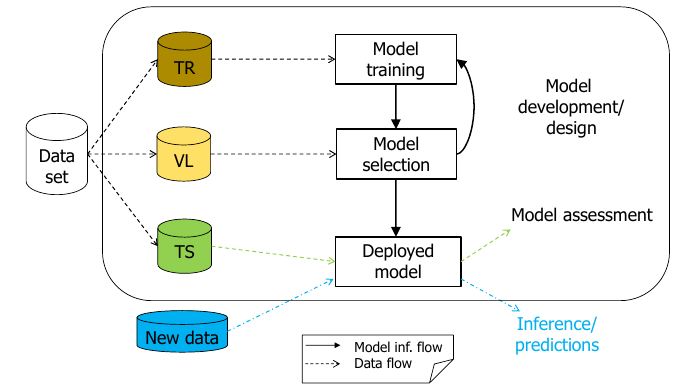
\includegraphics[width=\textwidth]{images/dataSet}
                        \end{figure}

Specificity = TN / (FP + TN)
Positive
 Negative
Positive
 TP
 FN
 (True Negative rate =1 -FPR)
Sensitivity = TP / (TP + FN)
Negative
 FP
 TN
(True Positive rate or Recall)
(Precison= TP/(TP+FP))
false positive (FP) :eqv. with
false alarm
Accuracy: % of correctly classified patterns = TP +TN / total
Note: for binary classif.: 50% correctly classified = “coin” (random guess) predictor!
Other topics:
• unbalanced data (e.g. 99% +)  trivial classifier exists ,

ROC curve
The diagonal corresponds
to the worst classificator.
Better curves have higher
AUC (Area Under the
Curve).

Specificity = TN / (FP + TN)
Positive
 TP
 FN
 TPr or Sensitivity = TP / (TP + FN)
Negative
 FP
 TN

 Data collection:
–
 adequately large and representative set of examples
for training and test the system
Data representation
– domain dependent, exploit prior knowledge of the
application expert
– Feature selection
– Outliers detection
– Other preprocessing: variable scaling, missing data,..
Often the most critical phase for an overall success!
Model choice:
– statement of the problem
– hypothesis formulation
• You must know the limits of applicability of your model
– complexity control

Building of the model (core of ML):
– through the learning algorithm using the
training data
Evaluation:
– performance = predictive accuracy !
\end{description}
VC dim theory analysis !!!

